\documentclass[12pt,a4paper,oneside]{ctexart}
\usepackage{amsmath,amsthm,amssymb,wrapfig,graphicx,float,tabularx}
\title{衍射实验报告}
\author{张博厚 PB22071354}
\date{\today}
\newcommand\specialsectioning{\par
  \setcounter{section}{0}%
  \setcounter{subsection}{0}%
  \renewcommand\thesection{\relax}}

\begin{document}
\specialsectioning
\maketitle
\tableofcontents
\newpage
\section{一.实验背景}
波在传播方向上遇到障碍物时,会偏离直线传播而绕过障碍物前进,这种现象称为衍射(diffraction).
在经典物理学中,波在穿过狭缝,小孔或圆盘之类的障碍物后会发生不同程度的弯散传播.假设将一个障碍物置放在光源和观察屏之间,则会有光亮区域与阴暗区域出现于观察屏,
而且这些区域的边界并不锐利,是一种明暗相间的复杂图样,即衍射图样.\\ \indent
光作为一种波,同样具有衍射现象,惠更斯-菲涅尔原理最早有效地揭示了光的衍射现象原理,为近代物理光学奠定了理论基础.
光的衍射现象是近代光学技术的实验基础,研究光的衍射现象,有助于理解光的波动性特征,加深对光的本质的认识.
\section{二.实验原理}
根据光源-障碍物-接收屏距离不同,衍射可分为夫琅禾费衍射和菲涅尔衍射两种,本实验研究夫琅禾费衍射.\par
当光源与接收屏都距离衍射屏无限远(或相当于无限远)时,所产生的衍射为夫琅禾费衍射,此时入射光和衍射光都是平行光.
在本实验中,为了进行适当的简化,使用He-Ne激光器作为光源,同时使观察屏远离狭缝,则此时入射光与衍射光都可视为平行光.\\
\subsection*{单缝夫琅禾费衍射的光强分布}\par
在单缝衍射中,依据惠更斯-菲涅尔原理,狭缝上各点都可视为发射子波的新波源,
其光强分布为:
\begin{equation}
    I_{\phi}=I_0\left(\frac{\sin u}{u}\right)^2,u=\pi a\frac{sin\phi}{\lambda}
\end{equation}
其中$a$为单缝宽度,$I_0$为入射光光强,$\phi$为衍射角,由(1)可知,当
\begin{equation}
    asin\phi=k\pi,k=\pm 1,\pm2,\pm3.......
\end{equation}
时,有$u=k\pi(k=\pm 1,\pm2,\pm3.......)$,即$I_{\phi}=0$,为暗条纹.此时由于$\phi$
很小,有$\sin\phi=\phi$,于是由(2)式以及几何关系,可得
\begin{equation}
    \frac{k\lambda}{a}=\frac{x_k}{L}
\end{equation}
实验中,测量出各级暗条纹中心距中央亮条纹的距离$x_k$及单缝与衍射屏的距离$L$,即可计算得出单缝的宽度$a$.\\

\subsection*{双缝夫琅禾费衍射的光强分布}\par
将单缝换成双缝,每条狭缝宽度仍为$a$,,中间不透光部分宽度为$b$,则双缝中心间距
$d=a+b$,屏上衍射角$\phi$处的光强为:
\begin{equation}
    I_{\phi}=4I_0\frac{\sin^2u}{u^2}\cos^2v
\end{equation}
其中$u=\pi a\frac{\sin \phi}{\lambda},v=\pi d\frac{\sin\phi}{\lambda}$ \par
式(4)表明,双缝夫琅禾费衍射图样是单缝衍射和双缝干涉这两个因素共同作用的结果.且出现
双缝干涉光强极大值的条件是
\begin{equation}
    v=n\pi,\mbox{即}d\sin\phi=n\lambda,\mbox{近似为}d\phi=n\lambda
\end{equation}
特别地,当$\frac{n}{k}=\frac{d}{a}$时,会出现缺级现象,即第$n$级干涉极大不会出现.由(5)式,
当满足:
\begin{equation}
    \frac{n\lambda}{d}=\frac{x_k}{L}
\end{equation}
时,光强出现极大值,在实验中测量各级亮条纹距离中央亮条纹的距离$x_k$以及双缝
与衍射屏的距离$L$,可计算出双缝中心间距$d$\\

\subsection*{圆孔夫琅禾费衍射的光强分布}\par
光通过小孔会发生衍射,形成明暗相间的条纹衍射图样.大约有$84\%$的能量集中在中央亮斑
,称为艾里(Airy)斑.艾里斑的角度与波长$\lambda$及小孔的直径$D$满足关系:
$\sin\theta=\frac{1.22\lambda}{D}$
\section{三.实验目的}
\noindent
1.对光学实验形成初步的感性认识,掌握光的衍射实验装置的搭建方法.\\
2.观察单缝,双缝,圆孔,光栅等衍射元件的夫琅禾费衍射现象,加深对光的衍射现象的理解.\\
3.归纳总结不同衍射元件的衍射光强分布特征.\\
4.利用衍射图样测量并计算衍射屏的结构参数.\\
\section{四.实验内容}
\subsection*{实验仪器}
本次实验所需的仪器为光学导轨及其附件,He-Ne激光器(波长为632.8nm)及电源,衰减片(用于调节光强),
衍射元件(单缝,双缝,圆孔,光栅等),CCD(作为接收屏并在显示屏上显示图案),显示屏,支架等.
\subsection*{实验步骤} \noindent
1.正确组装实验仪器,移动各仪器,调节光路水平,使得激光恰好射在CCD元件的正中央.\\
2.依次安装不同的衍射元件,观察并总结各元件衍射图样的特点.\\
3.更换不同缝宽(直径)的单缝/双缝/小孔,观察衍射图样的变化规律.\\
4.再次更换为单缝,记录中央主极大与各级暗条纹的位置.\\
5.更换为双缝,记录双缝衍射各级亮条纹的位置.\\
6.实验结束,整理实验器材,将各仪器及元件归位.\\
\section{五.实验数据与结论}
\subsection*{各元件衍射图样的特点及变化}
\noindent
1.单缝衍射:\par
如图1所示,单缝衍射图样是一系列明暗交错的条纹,中央亮条纹的光强最大且角宽度最大,
从中央向两侧延伸,各级亮条纹的宽度大致为中央亮条纹的$\frac{1}{2}$,且亮度从中央向两侧逐渐衰减.
\par
单缝衍射图样与单缝的宽度有关,当缝宽越大时,衍射条纹越细,即各级条纹的角宽度越小,因而衍射条纹越细锐.\\
\begin{figure}[H]
    \centering
    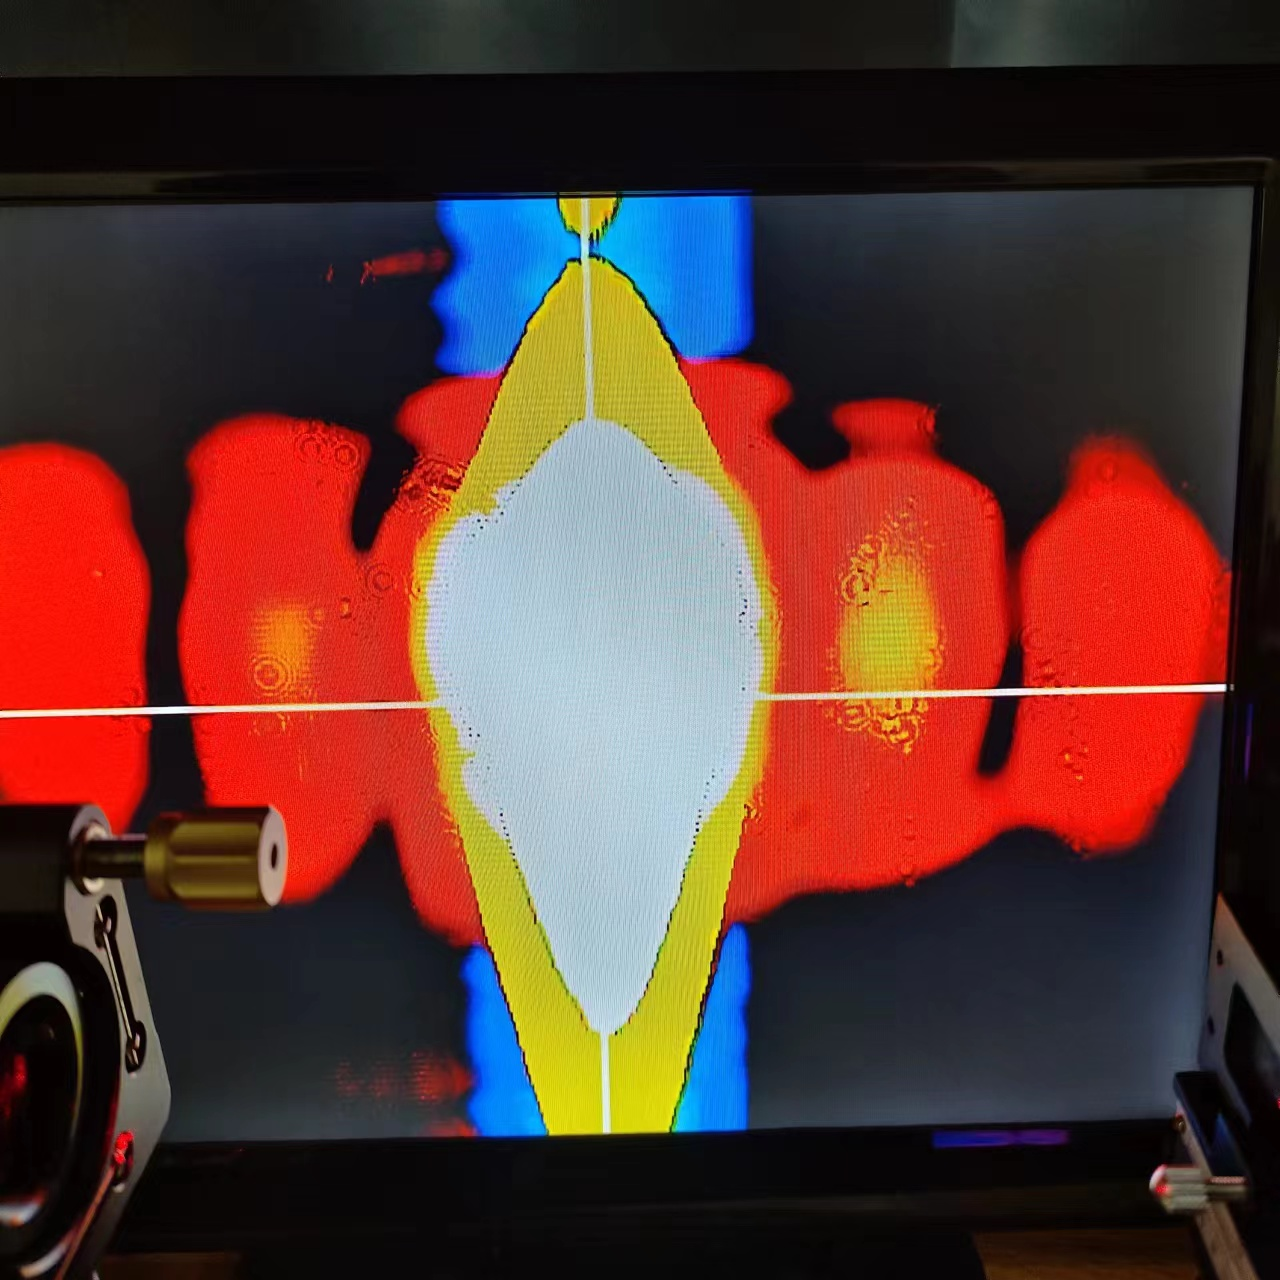
\includegraphics[scale=0.15]{df.jpg}
    \caption{单缝衍射图样}
\end{figure}
2.双缝衍射\par
如图2所示,中央条纹的亮度最大,两侧条纹关于中央对称,且亮度依次递减,条纹中的宽度近似相等,特别地.
由于双缝衍射中干涉与衍射现象同时存在,当干涉极大与衍射极小重合时,会出现缺级现象.
\par
更换不同中心间距的双缝元件,可以观察到不同的衍射图样,双缝中心间距$d$越小,则衍射现象
越明显,衍射条纹宽度越宽.此外,缺级现象出现的级数也与中心间距有关\\
3.圆孔衍射\par
如图3所示结果,夫琅禾费圆孔衍射在中央接收屏上显示的衍射图样是一系列的同心圆环,明暗交错,
其中最中央的衍射斑(即艾里斑)集中了最多的能量,从中央向两边延伸,光强逐渐减弱,
且不同级次的圆环之间角距离并不相等.
\par
换用不同直径的圆孔,可以观察到中央主极大(艾里斑)的宽度发生变化,且圆孔直径越大,艾里斑直径越小.

\begin{figure}[H]
    \begin{minipage}[t]{0.5\linewidth}
        \centering
        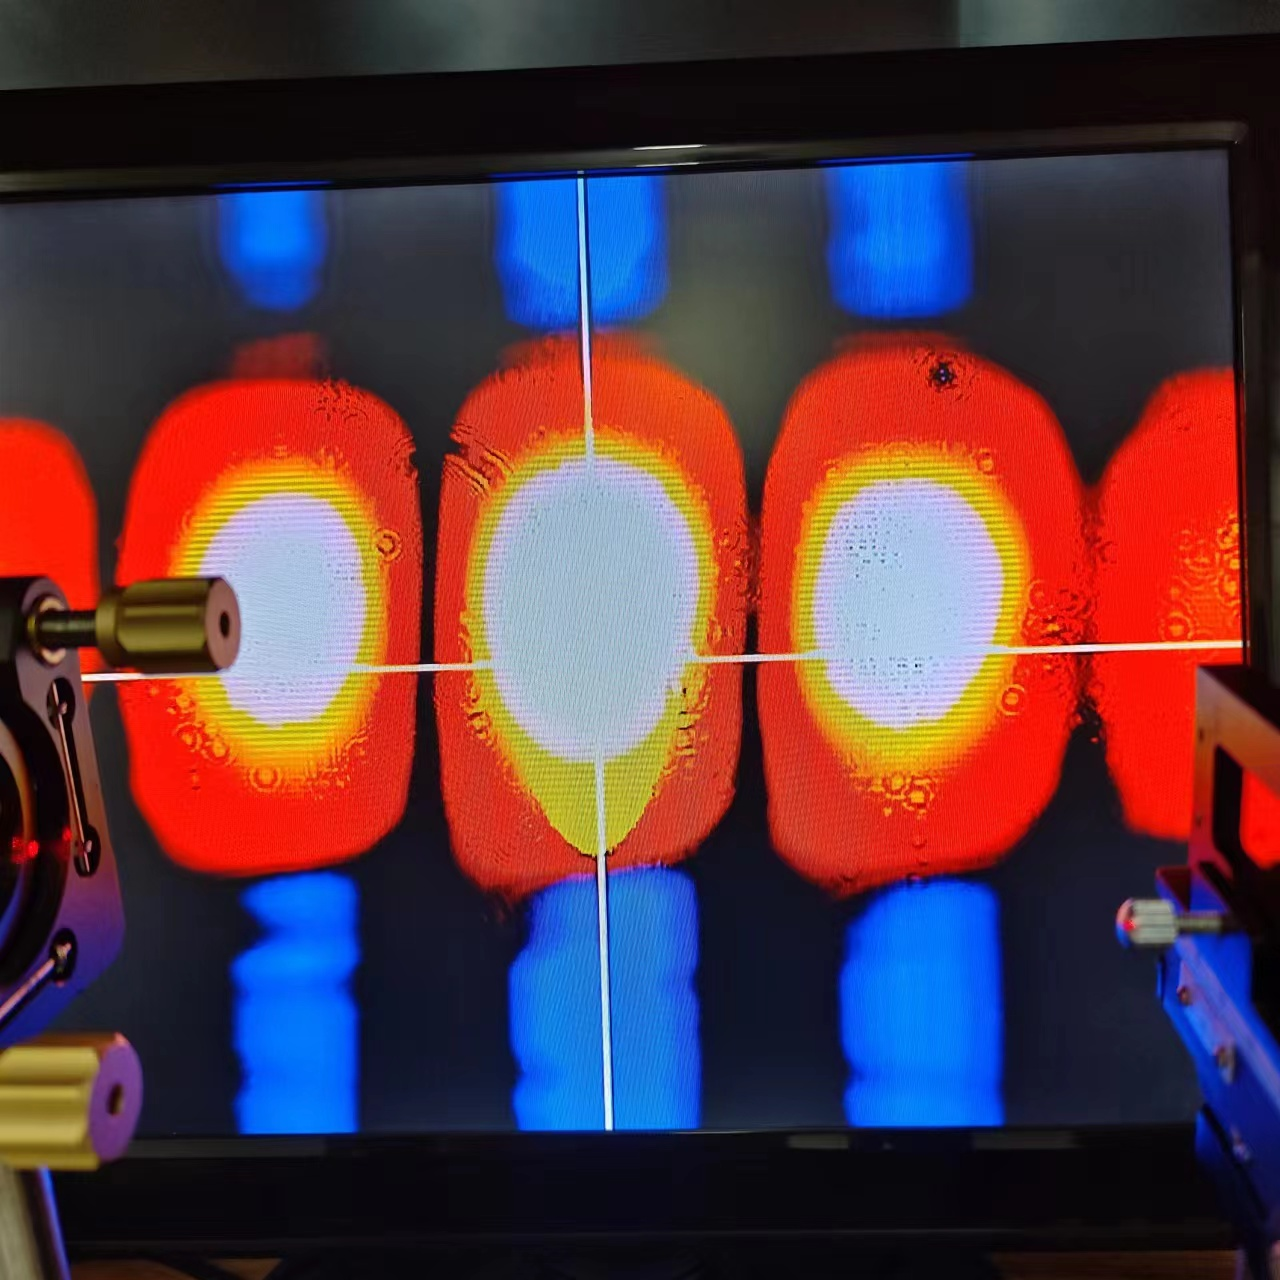
\includegraphics[scale=0.15]{sf.jpg}
        \caption{双缝衍射图样}
        \label{fig:side:a}
      \end{minipage}%
      \begin{minipage}[t]{0.5\linewidth}
        \centering
        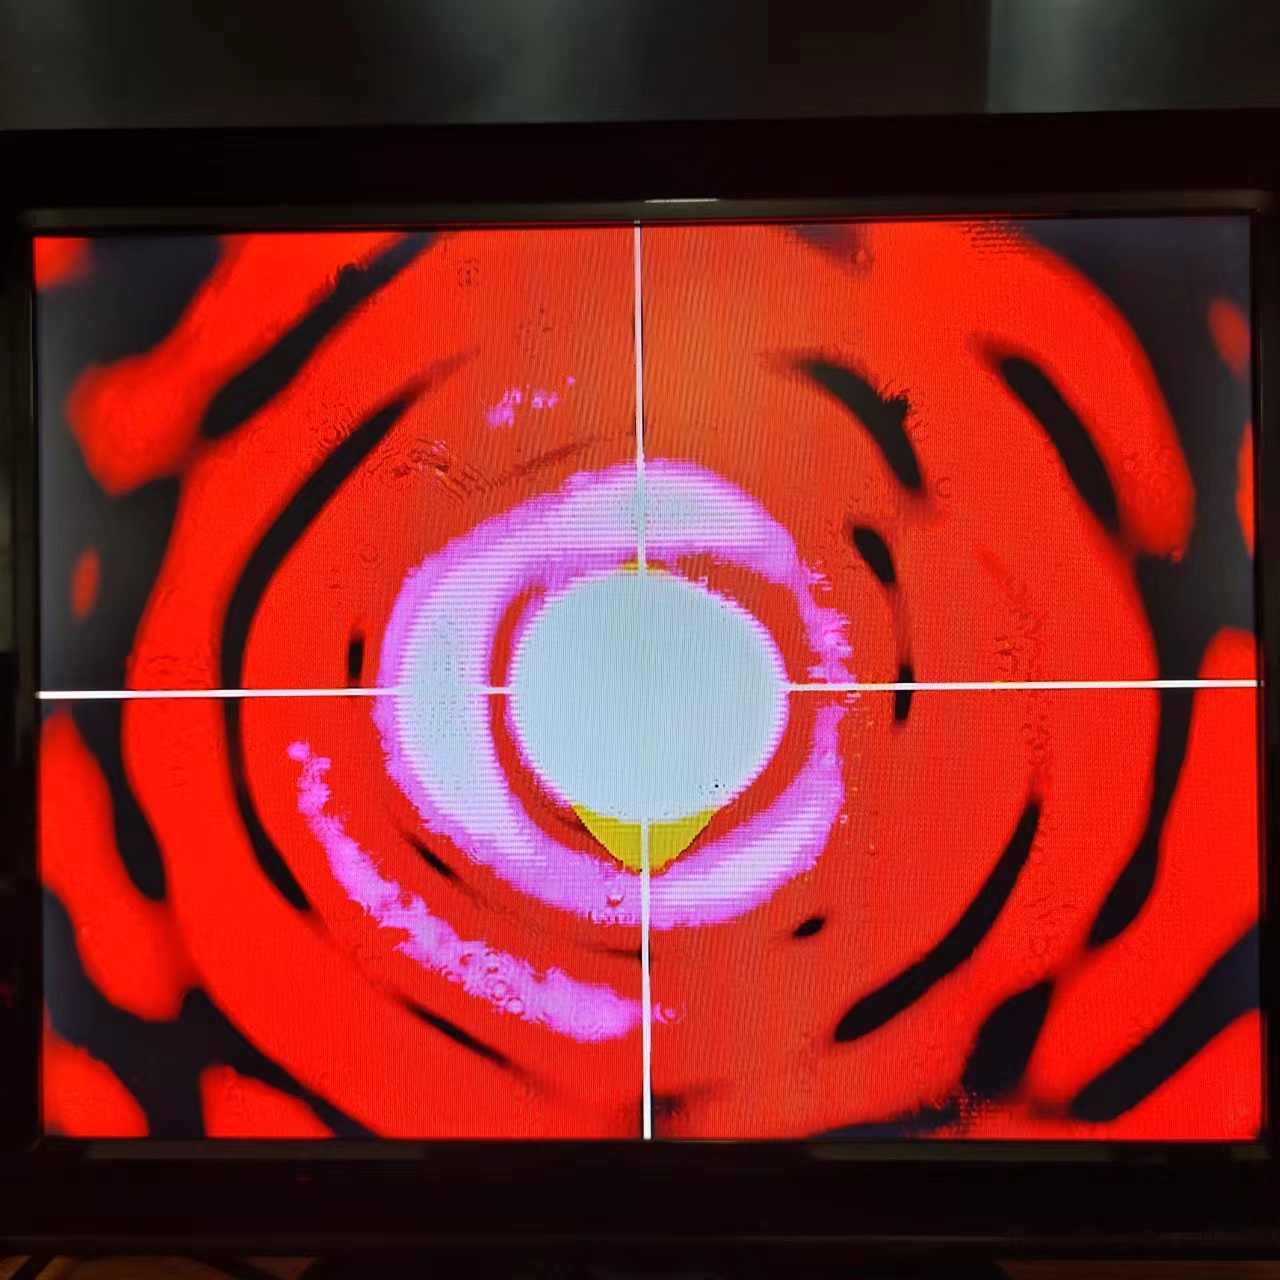
\includegraphics[scale=0.15]{yk.jpg}
        \caption{圆孔衍射图样}
        \label{fig:side:b}
      \end{minipage}
     
\end{figure}
\subsection*{数据处理与误差分析}
单缝衍射实验原始数据如下表(采用300$\mu m$单缝):
\begin{center}
    \begin{tabular}{|c|c|c|c|c|c|c|c|}
    \hline
    k&0&1&2&3&4&5&6\\
    \hline
    L/cm& 29.75& 29.75 & 29.75 & 29.75 & 29.75 & 29.75&29.75\\
    \hline
    $x_k$/mm&9.323&8.700&7.902&7.222&6.416&5.770&4.912\\
    \hline    
    $\Delta x_k$/mm&0&0.623&1.421&2.101&2.907&3.553&4.411\\
    \hline   
    \end{tabular}
\end{center}
计算$a$并求平均值,可得缝宽为
$$\overline{a}=269.33\mu m,\mbox{相对误差}\frac{\Delta a}{a}=10.2\%$$
双缝衍射实验原始数据如下表(使用$d=190\mu m$双缝):
\begin{center}
    \begin{tabular}{|c|c|c|c|c|c|c|c|c|c|c|}
    \hline
    k&0&1&2&3&4&5&6&7&8&9\\
    \hline
    L/cm& 29.75& 29.75 & 29.75 & 29.75 & 29.75 & 29.75&29.75&29.75&29.75&29.75\\
    \hline
    $x_k$/mm&8.950&9.985&10.970&缺级&12.350&13.362&缺级&15.331&16.335&缺级\\
    \hline    
    $\Delta x_k$/mm&0&1.035&2.020&缺级&3.400&4.412&缺级&6.381&7.385&缺级\\
    \hline   
    \end{tabular}
\end{center}
计算$d$并求平均值,可得双缝中心间距为
$$\overline{d}=188.66\mu m,\mbox{相对误差为}\frac{\Delta d}{d}=0.92\%$$
\textbf{误差分析:}\par
注意到单缝实验结果与真实值产生了较大误差,本实验中误差产生的原因可能为:\\
1.千分尺本身具有一定读取误差,在实验过程中注意到,由于设备老化,在旋转千分尺时偶尔会出现空程,使得仪器误差增大.\\
2.在实验开始之前,未调节光路至使之恰好直射传感器中央,有一定倾斜.\\
3.人眼具有一定的观察角,由于观察角度问题,对于明暗条纹中心的判断具有较大误差.\\
4.未调节光强为最合适值,使得光衍射后产生光晕,对结果产生影响.\\
5.实验室内的环境光对于衍射图样也有一定的影响.
 \section{六.思考与讨论}\noindent
 1.当光通过一个小孔时,在后面的光屏上会得到什么图案?
 \par 当小孔直径较大时,光沿直线传播,光屏上出现与小孔等大的光斑;缩小小孔的直径,
 会发生小孔成像,在光屏上形成光源的倒立的像;当小孔直径缩小至与光的波长相近时,发生衍射现象,
 在光屏上形成明暗相间的圆环.\\
 2.白光照射到狭缝上,衍射条纹有什么特点?\par
 白光是由几种不同的色光组成的,在通过狭缝时,由于不同色光的波长不同,由式(3),
 与中央主极大的距离$x_k$也不同,会观察到不同的彩色直条纹对称地排布在中央亮条纹两侧.且从中央向两侧,色光
 的波长依次变长,宽度逐渐变窄.\\
 3.解释LED射灯照到手机屏幕上的现象.\par
 手机屏幕可以视为一个光栅,当射灯照到手机屏幕时,光通过不同的狭缝向不同方向
 衍射,设光栅间距为$d$(在题设情境下与手机屏幕像素有关),则在衍射极大处满足
 $$d(\sin\phi\pm\sin i)=m\lambda,m=1,2,3......$$
上式表明衍射图样与波长有关,LED射灯发出的光是白光,含有不同波长的色光,
因此通过手机的光栅衍射作用会发生色散,形成如图中所示的图案.

\end{document}